\section{Results}\label{sec_results}

\subsection{Calculation of the grating constant}

In our case, we will calculate the grating constant $g$ using hypothetical values for the reasons mentioned in section~\ref{sec_methodology}.
By rearranging and combining eq.~\ref{eq_interference} and eq.~\ref{eq_phi} we find a formula for the grating constant~\ref{eq_g}.

\begin{align}
    g &= \frac{p \lambda}{\sin(\phi)} \label{eq_g}\\
    \phi &= \arctan \left( \frac{x}{D} \right)
\end{align}

To calculate the uncertainty of the grating constant, the Gaussian error propagation was used.
\begin{align}
    \Delta g &= \sqrt{{\left( \frac{\partial g}{\partial p} \Delta p \right)}^2 + {\left( \frac{\partial g}{\partial \lambda} \Delta \lambda \right)}^2 + {\left( \frac{\partial g}{\partial \phi} \Delta \phi \right)}^2}\\
    \Delta \phi &= \sqrt{{\left( \frac{\partial \phi}{\partial x} \Delta x \right)}^2 + {\left( \frac{\partial \phi}{\partial D} \Delta D \right)}^2}
\end{align}

The hypothetical value of the grating constant $g$ and its uncertainty can now be calculated:
\begin{align}
    \bf g = (1520 \pm 20) ~\si{\bf\nano\meter} = (1.52 \pm 0.02) ~\si{\bf\micro\meter} \label{res_g}
\end{align}

Note that the obtained value is not the real value and that a different value for the grating constant $g$~\cite{src_grating_constant} is used in the remaining calculations.

\subsection{Calculation of the distance between the grating and the camera}

As mentioned in the previous chapter, the first goal is to find the distance $d$ of the grating
and the image sensor.
By combining eq.~\ref{eq_interference} and eq.~\ref{eq_phi} we get the following equation for $d$:
\begin{align}
    d = \frac{x}{\tan(\phi)} = \frac{x}{\tan(\arcsin(\frac{\lambda}{g}))} \label{eq_distance}
\end{align}

Multiple steps are necessary to calculate the distance $d$.
First of all, we took a picture with the spectrometer pointed at the sunlight (fig.~\ref{fig_sunlight}). We then selected suitable 
points in the spectrum and compared them to tabulated wavelengths and their corresponding colors 
in fig.~\ref{fig_wavelengths}. In the next step, we measured the distance $x$ required in eq.~\ref{eq_distance} of said points to the zero-order maximum
using the imtools method in Matlab.

For our final calculation of the distance $d$, we averaged multiple measurement points to get a more
accurate result. This is shown in Fig.~\ref{fig_sunlight}.

The error calculations for eq.~\ref{eq_distance} were done using the Gaussian error propagation.
Please refer to our Jupyter notebook~\cite{GitHub}, for the full calculations of all the values and 
error propagations presented in this chapter. 
\begin{align}
    \Delta d = \sqrt{{\left(\frac{\partial d}{\partial x}\right)}^2 + {\left(\frac{\partial d}{\partial \lambda}\right)}^2}
\end{align}

Our average result for the distance $d$ is:
\begin{align}
    \bf d = (1.7 \pm 0.1) ~\si{\bf\milli\meter} \label{res_d}
\end{align}

We have now successfully calibrated our spectrometer and we can now determine the wavelength
of any point in the picture.
The following equation is used to determine the wavelength of a point with a certain pixel 
distance $x$ to the zero-order maximum.
\begin{align}
    \lambda = g \sin\left(\arctan\left(\frac{x}{d}\right)\right) \label{eq_lambda}
\end{align}

Again the uncertainties were determined using the Gaussian error propagation.
\begin{align}
    \Delta \lambda = \sqrt{{\left(\frac{\partial \lambda}{\partial x}\right)}^2 + {\left(\frac{\partial \lambda}{\partial d}\right)}^2}
\end{align}

\subsection{Analysis of different light sources}

Using these obtained results we analyzed some different types of light sources. In each case, we assumed 
an error of $\pm 10$ pixels, since we had to choose the position of each measurement point in the picture by hand.

First of all, we analyzed a fluorescent tube lamp. As can be seen in Fig.~\ref{fig_lamp1} below, this type of 
light source only emits certain small ranges of wavelength. In our case, we measured the following ranges:
\begin{alignat}{3}
    &\text{Red spectrum:} \; &&(587 \pm 36)~\si{\nano\meter} & &- (622 \pm 38)~\si{\nano\meter} \nonumber\\
    &\text{Green spectrum:} \; &&(487 \pm 32)~\si{\nano\meter} & &- (560 \pm 35)~\si{\nano\meter} \nonumber\\
    &\text{Blue spectrum:} \; &&(430 \pm 29)~\si{\nano\meter} & &- (455 \pm 31)~\si{\nano\meter} \nonumber
\end{alignat}
\vspace{-2em}
\begin{figure}[H]
    \centering
    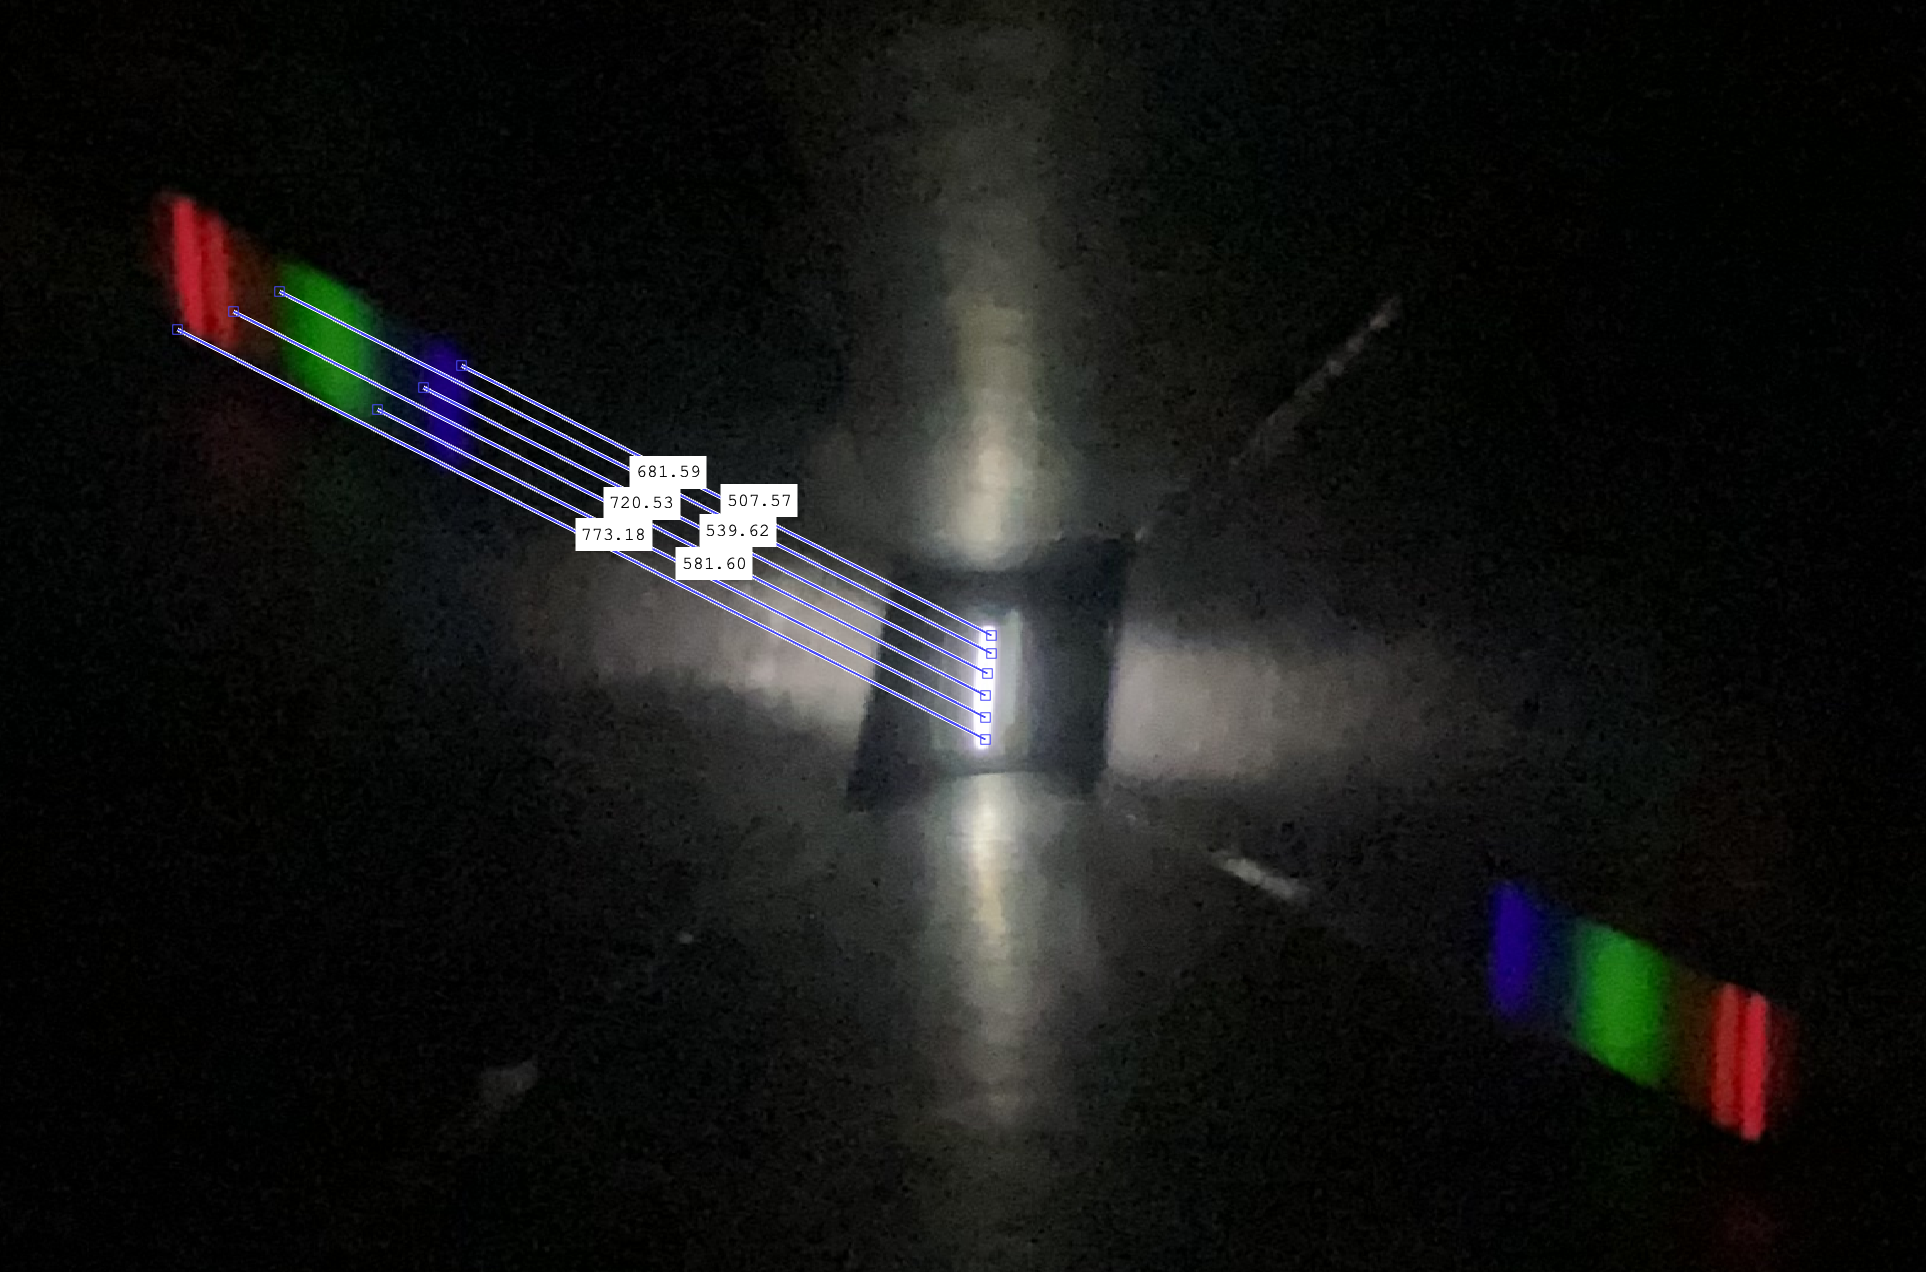
\includegraphics[scale = 0.28]{src/images/lamp1_meas.png}
    \caption{Spectrum of a fluorescent tube.}~\label{fig_lamp1}
\end{figure}

As a second example, we analyzed a LED ceiling lamp. As can be seen in Fig.~\ref{fig_lamp2} below, this lamp
emits almost the entire spectrum of visible light with no significant gaps. We measured the following range:
\begin{alignat}{3}
    &\text{Full spectrum:} \; &&(429 \pm 29)~\si{\nano\meter} & &- (650 \pm 38)~\si{\nano\meter} \nonumber
\end{alignat}
\vspace{-2em}
\begin{figure}[H]
    \centering
    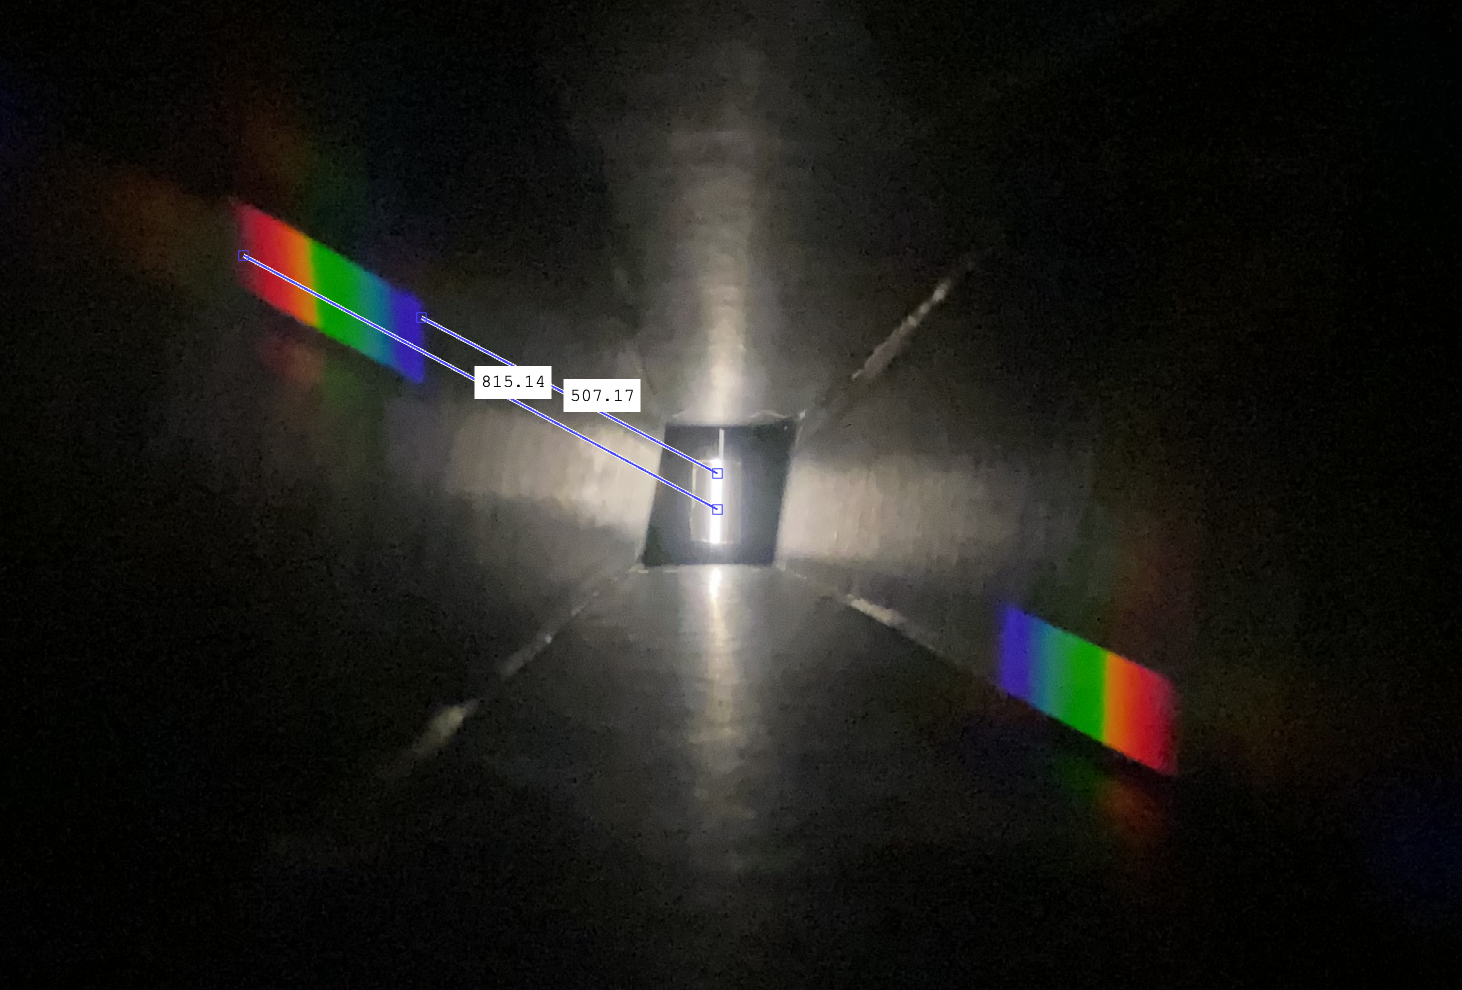
\includegraphics[scale = 0.38]{src/images/lamp2_meas.png}
    \caption{Spectrum of an LED ceiling light.}\label{fig_lamp2}
\end{figure}

Lastly, we analyzed the computer screen of a laptop. In this example, the color purple was shown on the screen.
As can be seen in Fig.~\ref{fig_purple_screen} only two very narrow bands of wavelengths are emitted.
\begin{alignat}{3}
    &\text{Red spectrum:} \; &&(597 \pm 37)~\si{\nano\meter} & &- (622 \pm 38)~\si{\nano\meter} \nonumber\\
    &\text{Blue spectrum:} \; &&(433 \pm 29)~\si{\nano\meter} & &- (457 \pm 37)~\si{\nano\meter} \nonumber
\end{alignat}
\begin{figure}[H]
    \centering
    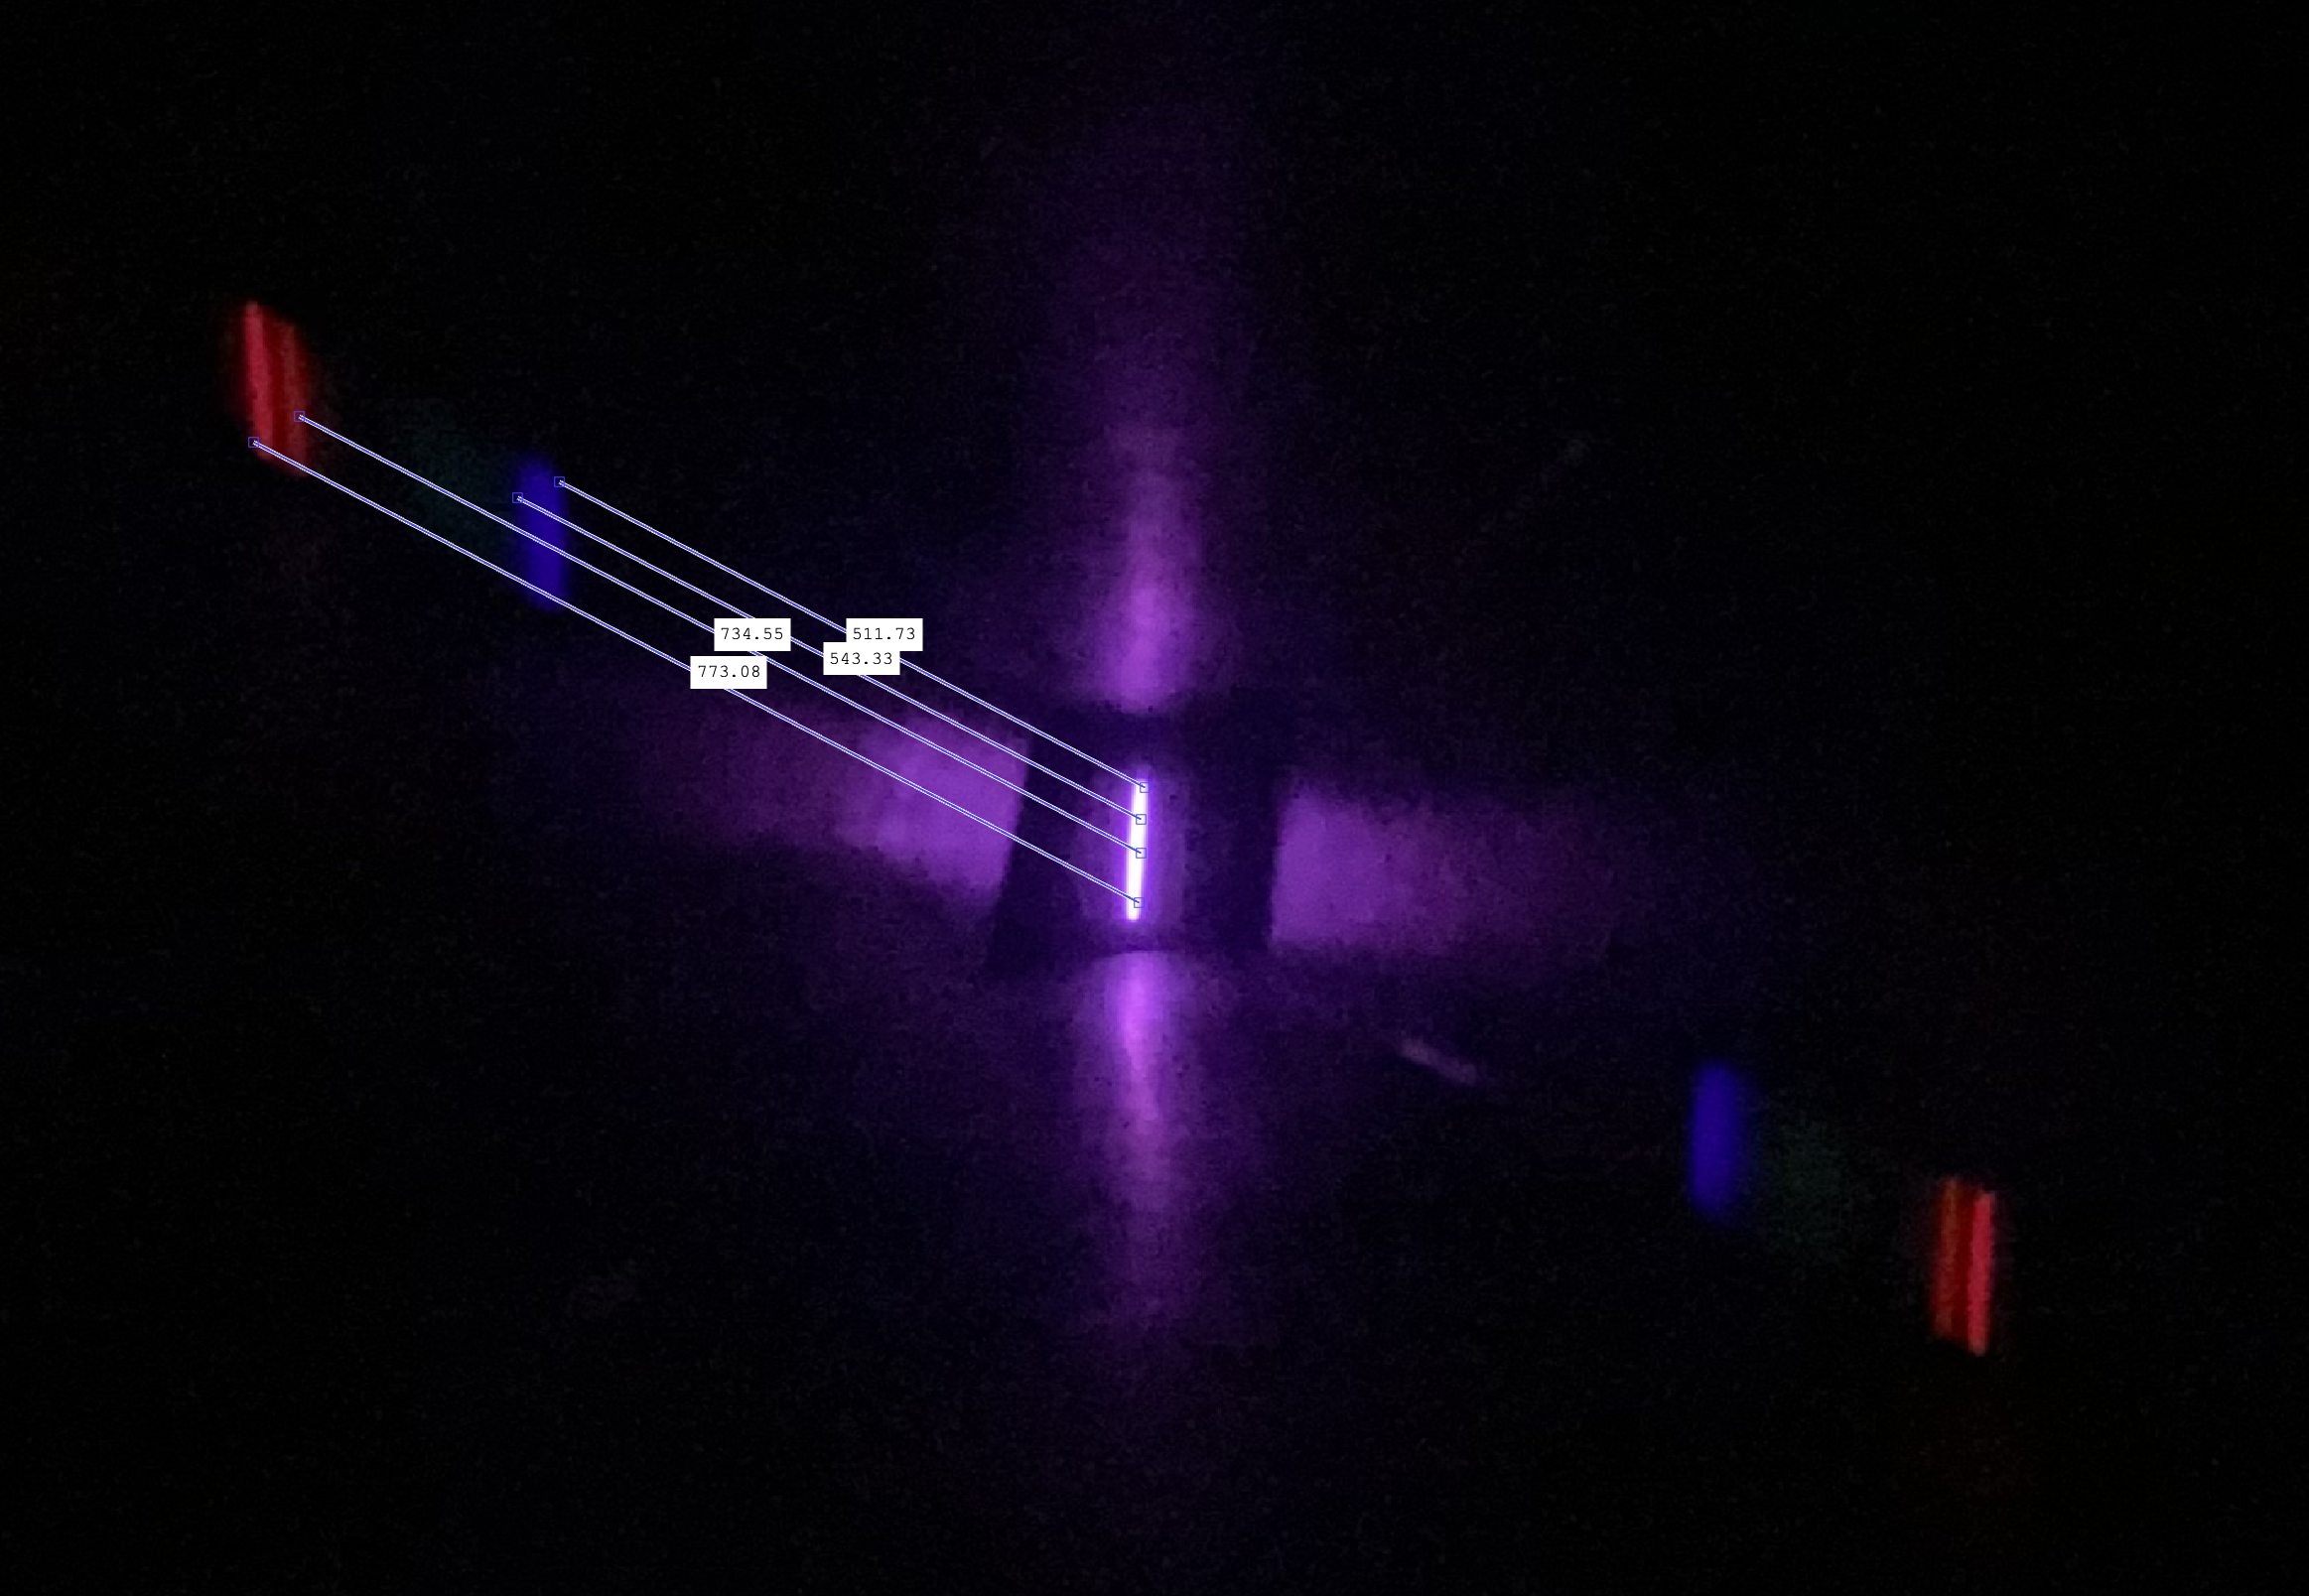
\includegraphics[scale = 0.24]{src/images/purple_screen_meas.png}
    \caption{Spectrum of a computer screen displaying a purple color.}\label{fig_purple_screen}
\end{figure}

Modern computer screens use LEDs as a light source. Typically the screen consists of many small red, blue and 
green LEDs that are located next to each other in a repeating pattern. Even though only a small fraction of 
the entire visible spectrum of light is emitted, these screens can reach a very high color accuracy. Our eyes 
contain three different types of receptors, that can detect different ranges of wavelengths corresponding 
to the colors red, green and blue. Our brain generates a color by mixing the information of these receptors, 
which is why the color on our screens seems natural to us.

\subsection{Theoretical spectra of light sources}

In the experiment 15 two different light sources were analyzed: A helium discharge tube, as well as
a mercury light. These are not commonly available types of light sources. Both lamps only emit very narrow bands
of wavelengths. We took the expected wavelength values from the literature, as cited below.

In the following figure~\ref{fig_helium_spectrum}, the expected wavelengths of a helium discharge tube are 
drawn into the spectrum of sunlight.~\cite{Helium Discharge Tube}
\begin{figure}[H]
    \centering
    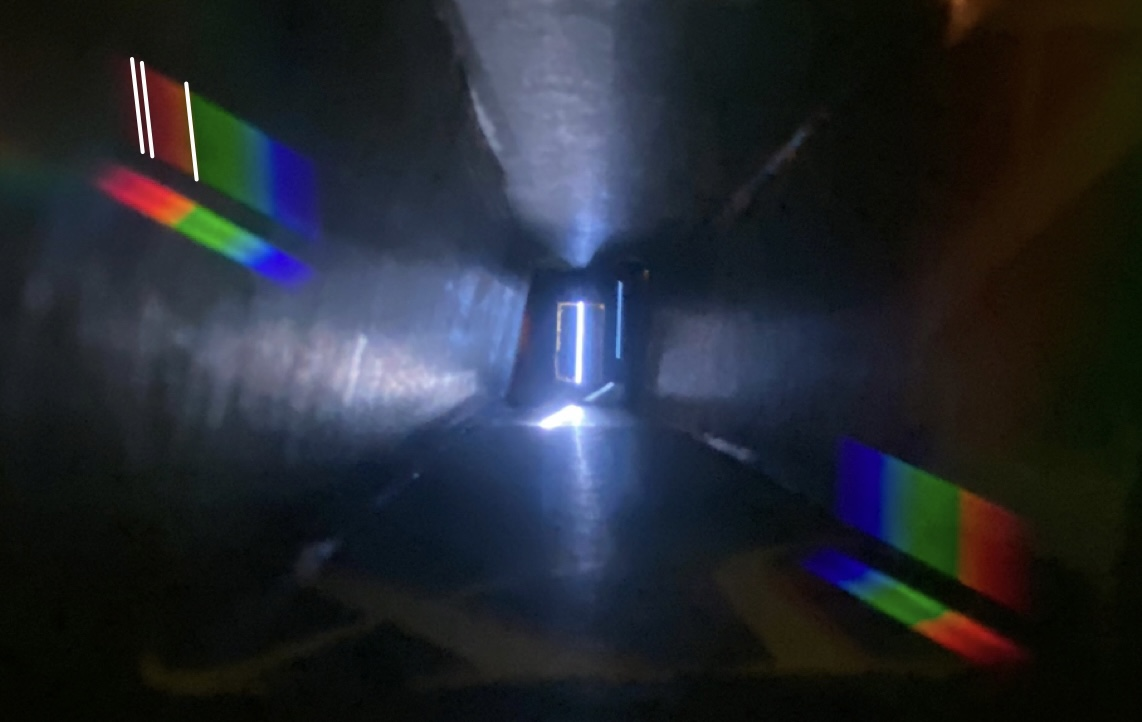
\includegraphics[scale = 0.23]{src/images/helium_spectrum.jpg}
    \caption{Expected helium spectrum is drawn in white color into the spectrum of sunlight.}\label{fig_helium_spectrum}
\end{figure}
\vspace{-1em}
Lastly in the following figure, the expected wavelengths of a mercury light are drawn into the spectrum of sunlight.~\cite{Mercury Vapor Lamp}
\begin{figure}[H]
    \centering
    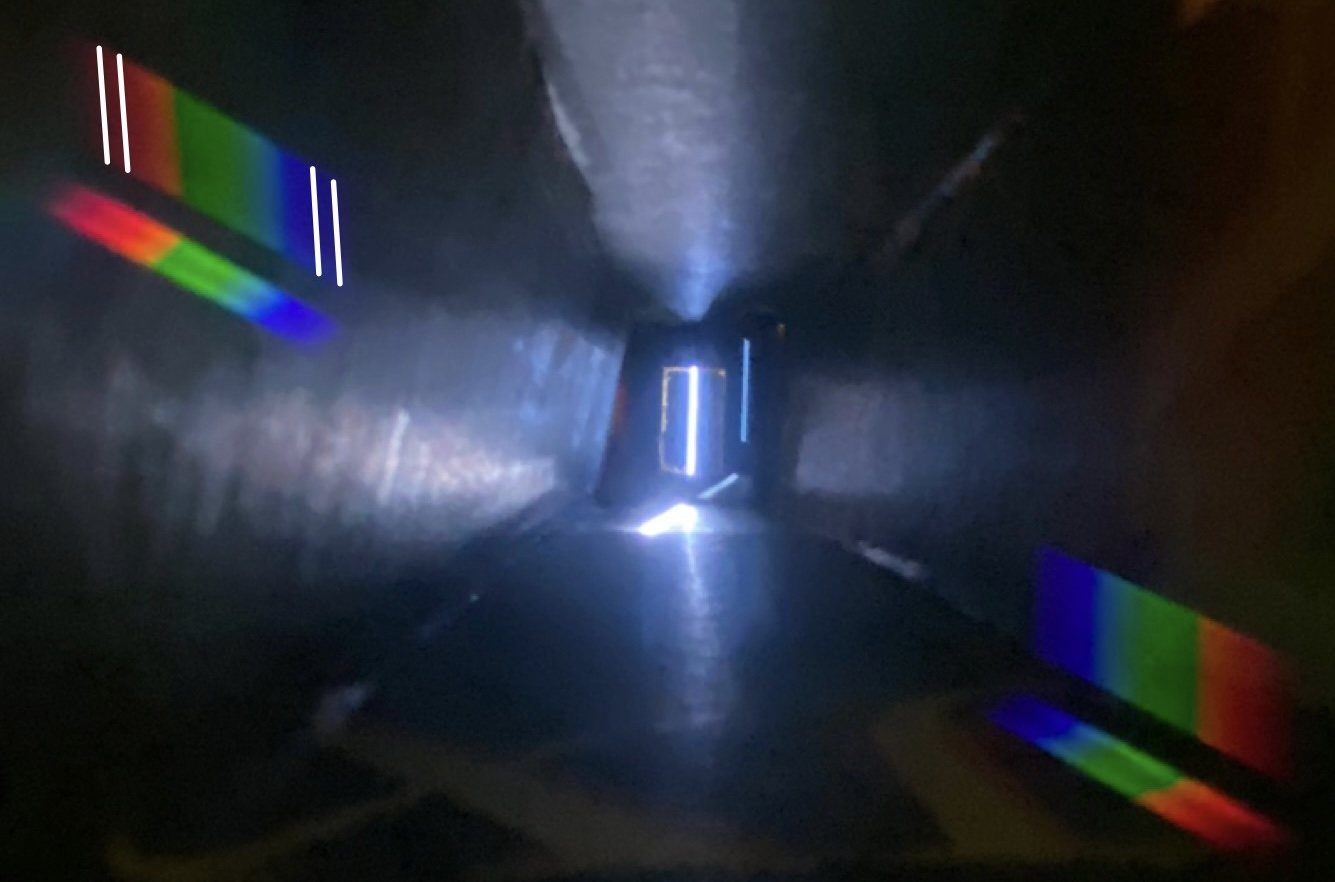
\includegraphics[scale = 0.2]{src/images/mercury_spectrum.jpg}
    \caption{Expected mercury spectrum is drawn in white color into the spectrum of sunlight.}\label{fig_mercury_spectrum}
\end{figure}